\documentclass[fontsize=15pt]{jlreq}

%プリアンブル 
\usepackage{tikz}
\usepackage{amsmath}
\usepackage{mathtools}
\pagestyle{empty}
\usepackage[top=15mm, bottom=20mm, left=20mm, right=20mm]{geometry}

%コマンド
\newcommand{\m}[1]{\raisebox{0.1em}{\textcircled{\scriptsize #1}}}


\begin{document}
\begin{center}
{\LARGE {振り返り}} \\
-物理\m{3}- %単元ごとに変えるか消す
\end{center}
\vspace{1em}
\begin{flushright}
名前：\underline{\hspace{5cm}}
\end{flushright}

\begin{enumerate}
\item 2つの力と同じはたらきをする一つの力をなんというか．\\
(\hspace{4cm})
\vspace{2em}

\item 力の合成を行うときの方法をかけ．\\
(\hspace{15cm})
\vspace{2em}

\item 1つの力を複数の力に分けたときの力をなんというか．\\
(\hspace{4cm})
\vspace{2em}

\item 次の図で示されているそれぞれの力の名称をかけ．また，重力の分力を斜面方向と，斜面垂直方向とに分けろ．(図に書き込む)\\[1em]
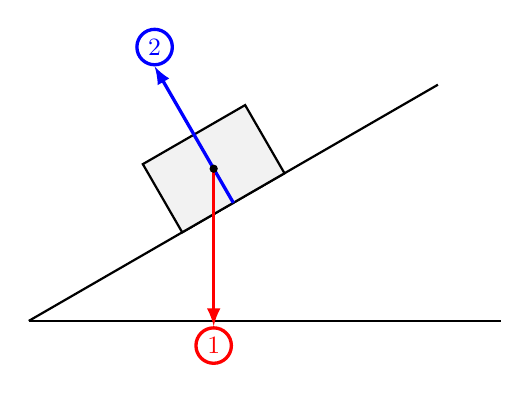
\begin{tikzpicture}[
    >=latex,
    num_label/.style={circle, draw, solid, inner sep=1pt, minimum size=4.5mm, font=\small, fill=white}
]
    \def\angle{30} 
    \def\boxW{1.5} 
    \def\boxH{1.0} 
    \def\boxPos{3} 
    \draw[thick] (0,0) -- (6,0); 
    \draw[thick] (0,0) -- (\angle:6); 
    \begin{scope}[rotate=\angle]
        \coordinate (Center) at (\boxPos, \boxH/2);
        \coordinate (BottomMid) at (\boxPos, 0);
        \draw[thick, fill=gray!10] 
            (\boxPos-\boxW/2, 0) rectangle (\boxPos+\boxW/2, \boxH);
        \draw[->, very thick, blue] (BottomMid) -- ++(0, 2) node[above, num_label, text=blue] {2};
    \end{scope}
    \draw[->, very thick, red] (Center) -- ++(0, -2) node[below, num_label, text=red] {1};
    \fill (Center) circle (1.5pt);

\end{tikzpicture}\\
\m{1}\\[0.5em]
\m{2}
\vspace{2em}

\item 4の問題では，それぞれなんの力が釣り合っているか．
\begin{itemize}
    \item 
    \item
\end{itemize}

\end{enumerate}
\end{document}
